\documentclass{article}
\usepackage[utf8]{inputenc}
\usepackage{tabu}
\usepackage{pgf}
\usepackage{tikz}
\usepackage{geometry}
\geometry{letterpaper}
\usepackage{graphicx}
\usepackage{mathtools}
\usepackage{caption}
\usepackage{subcaption}
\usepackage{amssymb}
\usepackage{hyperref}
\usepackage{enumitem}
\usepackage{listings}
\usepackage{float}
\usepackage[utf8]{inputenc}
\usepackage[english]{babel}
\author{Quentin Vilchez, Fin Vermehr and Binderiya Adishaa}
\title{Proposal}
\begin{document}
\maketitle
\usetikzlibrary{arrows,automata}
\section{Goal:}
\begin{itemize}
\item Our goal is to better understand how news spread on a social network, in our case we wish to focus on twitter. \\
We would like to apply a compartment model similar to the SIR model.
\item Our question would be:
\\ \textit{How does the existence of a susceptible population, with a history of infection by similar topics, modify the outbreak of a story on a social media?}
\end{itemize}


\section{Our Approach:}
\begin{itemize}
\item There has been some work done on this topic, specifically by Bettencourt et al. [1], who developped the SEIZ (Susceptibles Exposed Infectives Skeptics) model to describe the adoption of the Feynman diagrams by the scientific community around the world. This model introduced an exposed state and skeptic state, individuals in the exposed state take some time before they begin to believe/react to a story, individuals in the skeptics state do not believe the information and will not react to it. Furthermore, Fang Jin et al. [2] used this model to describe how information propagates on Twitter and demonstrated how this model is able to accurately capture the patterns in the spread of new/rumors on Twitter. 
\item  We would like to base ourselves on the work these\textit{ individuals}, and in a similar manner to Fang Jin et al. [2] describe how information spreads on Twitter. However, we think that it could be interesting to make a change to the model, by introducing a second susceptible population, which would account for people who have a history of tweeting about topics similar to the one in question. For example, if we study how the \#parkdaleshoting propagates on Twitter, similar topics would be \#guncontrol, \#NRA, etc. So people in the second susceptible population would be people who have tweeted about these topics in the past. \\
The reason for introducing this second population is that we feel that this second population has much more significant influence on the virality of certain content. Meaning that a story might become viral in a shorter span of time if there is a large second population and also they might cause other surrounding topics to go viral again. 
\\That is why we would like to focus on two stories, one with a large second population and one with a small second population. We believe, that the outbreaks will be different and that this can be described by our model. We will also compare our model to the simple SEIZ, to determine whether ours can fit the data better.

\item These are the equations that will describe our system:
\begin{equation} 
\begin{split}
\frac{dS_1}{dt} &= -{\beta}_1 S_1\frac{I}{N} -\gamma S_1\frac{Z}{N}\\
\frac{dS_2}{dt} &= -{\beta}_2 S_2\frac{I}{N}\\
\frac{dI}{dt} &= {\beta}_1 (1-p)S_1\frac{I}{N} + {\beta}_2 (1-m)S_2\frac{I}{N} + \epsilon E + \mu E\frac{I}{N}\\
\frac{dE}{dt} &= {\beta}_1 pS_1\frac{I}{N} + {\beta}_2 mS_2\frac{I}{N} + \gamma       lS_1\frac{Z}{N} - \mu E\frac{I}{N} - \epsilon E\\
\frac{dZ}{dt} &=  \gamma (1-l)S_1\frac{Z}{N}
\end{split}
\end{equation}
with,
\begin{align*}
 N& = S_1 + S_2 + E + Z + I & {\beta}_1 &< {\beta}_2  & 0\leq m<p\leq 1\\
0&\leq l \leq 1  & \frac{dN}{dt}&=0
\end{align*}
\end{itemize}
\section{Gathering data and analysis:}
\begin{itemize}
\item We have been gathering large amounts of data from Twitter. We will use this data in order to:
\begin{enumerate}
\item Create hashtag clusterings. These clusterings will allow us to see and understand what topics are close in nature, to the topic that we are trying to describe. These clusterings will also enable us to determine an approximate size for the second susceptible population at $t=0$ and hence the size of the first susceptible population at $t=0$ as well.
\\To cluster hashtags we have developped two algorithms based on the work of Ali Javed [3] on semantic hashtag clustering in social media. 
\item Fit the data to the equations. For that we will follow what Fang Jin et al. [2] did. 
\begin{figure}[h]

\centering
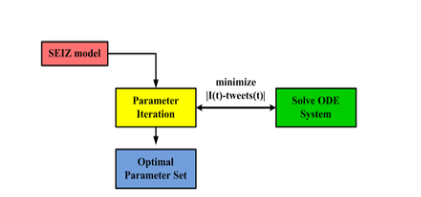
\includegraphics[width=0.5\textwidth]{/Users/quentinvilchez/Documents/GitHub/twitter-ideas-spread/workflow.png}
\caption{Numerical implementation work-flow.}
\end{figure}
\end{enumerate}

\end{itemize}
\section{Expected Results}
T
\section{References}
\begin{enumerate}[label={[\arabic*]}]
\item  L. Bettencourt, A. Cintron-Arias, D. I. Kaiser, and C. Castillo-Chavez. The power of a good idea: Quantitative modeling of the spread of ideas from epidemiological models. PHYSICA A, 364:513–536, 2006.
\item F. Jin, E. Dougherty, P. Saraf, Y. Cao, N. Ramakrishnan. Epidemiological Modeling of News and Rumors on Twitter, SNAKDD '13 Proceedings of the 7th Workshop on Social Network Mining and Analysis
Article No. 8.
\item A. Javed. A Hybrid Approach to Semantic Hashtag Clustering in Social Media, Graduate College Dissertations and  theses, 2016.
\end{enumerate}
\end{document}